\documentclass[a4paper,12pt]{article} % тип документа

% Поля страниц
\usepackage[left=2.5cm,right=2.5cm,
    top=2cm,bottom=2cm,bindingoffset=0cm]{geometry}
 

\DeclareUnicodeCharacter{2206}{$\Delta$}
\DeclareUnicodeCharacter{03C1}{$\rho$}

%Отступ после заголовка    
\usepackage{indentfirst}


% Рисунки
\usepackage{floatrow,graphicx,calc}
\usepackage{wrapfig}

% Создаёем новый разделитель
\DeclareFloatSeparators{mysep}{\hspace{1cm}}

% Ссылки?
\usepackage[unicode, pdftex]{hyperref} % подключаем hyperref
\usepackage{hyperref}
\usepackage[rgb]{xcolor}
\hypersetup{				% Гиперссылки
    colorlinks=true,       	% false: ссылки в рамках
	urlcolor=blue          % на URL
}


%  Русский язык
\usepackage[T2A]{fontenc}			% кодировка
\usepackage[utf8]{inputenc}			% кодировка исходного текста
\usepackage[english,russian]{babel}	% локализация и переносы


% Математика
\usepackage{amsmath,amsfonts,amssymb,amsthm,mathtools}


% Что-то 
\usepackage{wasysym}

\begin {document}

\begin{titlepage}
\newcommand{\HRule}{\rule{\linewidth}{0.3 mm}} % Defines a Hnew command for the horizontal lines, change thickness here

\center % Center everything on the page
 
%----------------------------------------------------------------------------------------
%	HEADING SECTIONS
%----------------------------------------------------------------------------------------

\textsc{\Large Московский физико-технический институт }\\[1.5cm] % Name of your university/college
\textsc{\Large Факультет аэрокосмических технологий}\\[0.5cm] % Major heading such as course name
\textsc{\large Лабораторная работа 2.5.1}\\[0.5cm] % Minor heading such as course title

%----------------------------------------------------------------------------------------
%	TITLE SECTION
%----------------------------------------------------------------------------------------

\HRule \\[0.4cm]
{ \huge \bfseries Измерение коэффициента поверхностного натяжения жидкости }\\[0.4cm] % Title of your document
\HRule \\[1.5cm]
 
%----------------------------------------------------------------------------------------
%	AUTHOR SECTION
%----------------------------------------------------------------------------------------

\begin{minipage}{0.4\textwidth}
\begin{flushleft} \large
\emph{Автор:}\\ Артем \textsc{Овчинников} % Your name
\end{flushleft}
\end{minipage}
\begin{minipage}{0.4\textwidth}
\begin{flushright} \large
\emph{Преподаватель:} \\
Арина Владимировна \textsc{Радивон} % Supervisor's Name
\end{flushright}
\end{minipage}\\[4cm]
%	DATE SECTION
%----------------------------------------------------------------------------------------

{\large \today}\\[2cm] % Date, change the \today to a set date if you want to be precise

%----------------------------------------------------------------------------------------
%	LOGO SECTION
%----------------------------------------------------------------------------------------

 
%----------------------------------------------------------------------------------------

\vfill % Fill the rest of the page with whitespace

\end{titlepage}
\tableofcontents
\newpage
\section{Аннотация}

Цель работы: 1) измерение температурной зависимости коэффициента поверхностного
натяжения дистиллированной воды с использованием известного коэффициента
поверхностного натяжения спирта; 2) определение полной поверхностной энергии и
теплоты, необходимой для изотермического образования единицы поверхности жидкости
при различной температуре. \\
В работе используются: прибор Ребиндера с термостатом и микроманометром;
исследуемые жидкости; стаканы.

\section{Теоретические сведения}

Наличие поверхностного слоя приводит к различию давлений по разные стороны от
искривленной границы раздела двух сред. Для сферического пузырька с воздухом внутри
жидкости избыточное давление даётся формулой Лапласа:
\begin{equation}
    \Delta P = P_\text{внутри} - P_\text{снаружи} = \frac{2\sigma}{r}
\end{equation}
где $ \sigma $ – коэффициент поверхностного натяжения, $ P_\text{внутри} $ и $ P_\text{снаружи} $ – давление внутри
пузырька и снаружи, $ r $ – радиус кривизны поверхности раздела двух фаз. Эта формула
лежит в основе предлагаемого метода определения коэффициента поверхностного
натяжения жидкости. Измеряется давление $ \Delta P $, необходимое для выталкивания в
жидкость пузырька воздуха.

\section{Методика измерений}

Обе погрешности можно устранить, погрузив кончик трубки до самого дна. Полное
давление, измеренное при этом микроманометром, $ P = \Delta P + \rho gh $. Заметим, что $ \rho gh $ от
температуры практически не зависит, так как подъём уровня жидкости компенсируется
уменьшением её плотности (произведение $ \rho h $ определяется массой всей жидкости и
поэтому постоянно). Величину $ \rho gh $ следует измерить двумя способами. Во-первых,
замерить величину $ P_1 = \Delta P^{'} $, когда кончик трубки только касается поверхности жидкости.
Затем при этой же температуре опустить иглу до дна и замерить $ P_2 = \rho gh + \Delta P" $ ($ \Delta P', \Delta P" $ –
давление Лапласа). Из-за несжимаемости жидкости можно положить $ \Delta P'= \Delta P " $ и тогда
$ \rho gh = P_2-P_1 $. Во-вторых, при измерениях $ P_1 $ и $ P_2 $ замерить линейкой глубину погружения
иглы $ h $.
Это можно сделать, замеряя расстояние между верхним концом иглы и любой
неподвижной частью прибора при положении иглы на поверхности и в глубине колбы. \\

\section{Используемое оборудование}

Исследуемая жидкость (дистиллированная вода)
наливается в сосуд (колбу) В (рис.1). Тестовая жидкость (этиловый спирт) наливается в
сосуд Е. При измерениях колбы герметично закрываются пробками. Через одну из двух
пробок проходит полая металлическая игла С. Этой пробкой закрывается сосуд, в
котором проводятся измерения. Верхний конец иглы открыт в атмосферу, а нижний
погружен в жидкость. Другой сосуд герметично закрывается второй пробкой. При
создании достаточного разряжения воздуха в колбе с иглой пузырьки воздуха начинают
пробулькивать через жидкость. Поверхностное натяжение можно определить по величине
разряжения $ \Delta P $ (1), необходимого для прохождения пузырьков (при известном радиусе
иглы). \\
Разряжение в системе создается с помощью аспиратора А. Кран К2 разделяет две полости
аспиратора. Верхняя полость при закрытом кране К2 заполняется водой. Затем кран К2
открывают и заполняют водой нижнюю полость аспиратора. Разряжение воздуха
создается в нижней полости при открывании крана К1, когда вода вытекает из неё по
каплям. В колбах В и С, соединённых трубками с нижней полостью аспиратора, создается
такое же пониженное давление. Разность давлений в полостях с разряженным воздухом и
атмосферой измеряется спиртовым микроманометром (устройство микроманометра
описано в Приложении). \\
Для стабилизации температуры исследуемой жидкости через рубашку D колбы В
непрерывно прогоняется вода из термостата. \\

\thisfloatsetup{floatrowsep=mysep}	
\begin{figure}[h!]
\begin{floatrow}
 \ffigbox[\FBwidth]{\caption{{{Схема установки для измерения температурной зависимости коэффициента поверхностного
натяжения}}}\label{fig:Graph_5}}%
         {\includegraphics[width=12cm,height=10.5cm]{physlabwork_13week_setup.png}}     
\end{floatrow}
\end{figure}

Обычно кончик иглы лишь касается поверхности жидкости, чтобы исключить влияние
гидростатического давления столба жидкости. Однако при измерении температурной
зависимости коэффициента поверхностного натяжения возникает ряд сложностей. Во-
первых, большая теплопроводность металлической трубки приводит к тому, что
температура на конце трубки заметно ниже, чем в глубине жидкости. Во-вторых, тепловое
расширение поднимает уровень жидкости при увеличении температуры. \\

\section{Результаты измерений и обработка данных}

Оцените погрешность измерения давления и температуры. Рассчитайте величину
коэффициента поверхностного натяжения воды $ \sigma (T) $, используя значение диаметра иглы,
полученное при измерениях на спирте (или измеренное на микроскопе).

\floatsetup[table]{capposition=top}	
\begin{table}[H]
	\caption{Результаты измерений}
	\label{table:main}
\begin{tabular}{lllllll}
T, C & T (error)           & $\Delta h $, mm & $ \Delta h $ (error) & $ \Delta P $, Pa & $ \sigma $, mN/m & $ \sigma $, mN/m (error) \\
23   & 0.004 & 86                          & 0.012              & 169      & 57     & 8.5     \\
25.6 & 0.004          & 84                          & 0.012              & 165      & 55     & 8.3     \\
30.5 & 0.003 & 85                          & 0.012              & 167       & 56     & 8.4     \\
35.3 & 0.003  & 82                          & 0.012              & 161      & 54     & 8.1      \\
40.1 & 0.002 & 82                        & 0.012              & 160     & 54    & 8.0     \\
45   & 0.002 & 80                          & 0.013                          & 157       & 53      & 7.9     \\
50   & 0.002               & 78                        & 0.013              & 152     & 51    & 7.6     \\
55   & 0.002 & 77                          & 0.013               & 151      & 51     & 7.6     \\
60   & 0.002 & 76                          & 0.013              & 149      & 50     & 7.5    
\end{tabular}
\end{table}

Постройте график зависимости $ \sigma (T) $ и определите по графику температурный
коэффициент $ d \sigma / dT $. Оцените точность результата.

\thisfloatsetup{floatrowsep=mysep}	
\begin{figure}[h!]
\begin{floatrow}
 \ffigbox[\FBwidth]{\caption{{{График зависимости $ \sigma (T) $}}}\label{fig:Graph_5}}%
         {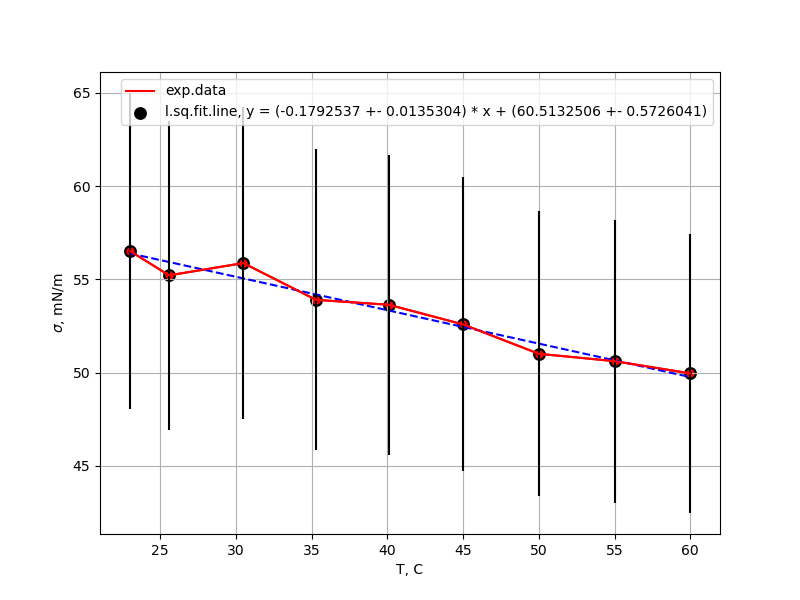
\includegraphics[scale=0.75]{physlabwork_13week_dsigmadT.png}}     
\end{floatrow}
\end{figure}

\begin{equation*}
    \frac{d \sigma}{dT} = -0.18 \pm 0.04
\end{equation*}

\newpage
На другом графике постройте зависимость от температуры \\
а) теплоты образования единицы поверхности жидкости $ q = - T \frac{d \sigma}{dT}$
б) поверхностной энергии U единицы площади F: $ \frac{U}{F} = ( \sigma - T \frac{d \sigma}{dT})$

\thisfloatsetup{floatrowsep=mysep}	
\begin{figure}[h!]
\begin{floatrow}
 \ffigbox[\FBwidth]{\caption{{{График зависимости q(T)}}}\label{fig:Graph_5}}%
         {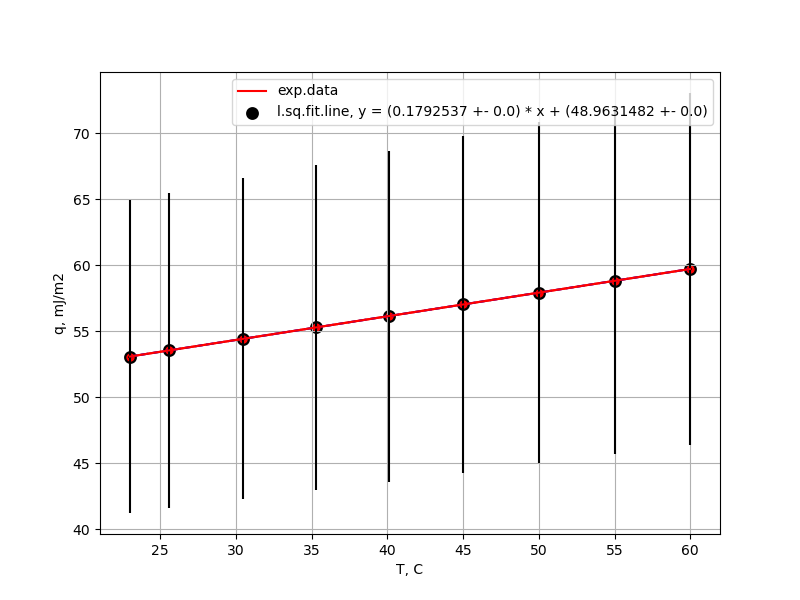
\includegraphics[scale=0.65]{physlabwork_13week_dqdT.png}}     
\end{floatrow}
\end{figure}

\thisfloatsetup{floatrowsep=mysep}	
\begin{figure}[h!]
\begin{floatrow}
 \ffigbox[\FBwidth]{\caption{{{График зависимости U/F(T)}}}\label{fig:Graph_5}}%
         {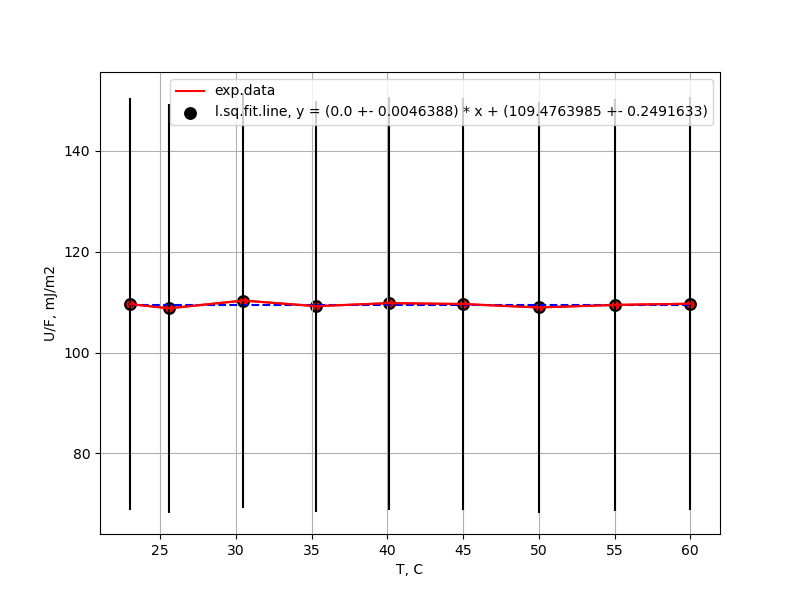
\includegraphics[scale=0.65]{physlabwork_13week_dUFdT.png}}     
\end{floatrow}
\end{figure}

\section{Обсуждение результатов}
На графике 2 видно, что поверхностное натяжение убывает с температурой линейно (что вдали от критической точки соотвествует теории). На графике 3 видно, что теплота образования единицы поверхности жидкости увеличивается с температурой линейно (что вдали от критической точки соотвествует теории). На графике 4 видно, что поверхностная энергия остается постоянной при увеличении температуры (что вдали от критической точки соотвествует теории).
\section{Выводы}
Вдали от критической температуры поверхностное натяжение с увеличением температуры убывает линейно. \\

Вдали от критической температуры теплота образования единицы поверхности жидкости с увеличением температуры увеличивается линейно. \\

Вдали от критической температуры поверхностная энергия с увеличением температуры остается постоянной.
\end{document}
